\documentclass[a4paper, 12pt]{article}
\usepackage[utf8]{inputenc}
\usepackage[english,russian]{babel}
\usepackage[warn]{mathtext}
\usepackage{graphicx}
\usepackage{float}
\restylefloat{table}
\usepackage{amsmath}
\usepackage{floatflt}
\usepackage[T2A]{fontenc}
\usepackage[left=20mm, top=20mm, right=20mm, bottom=20mm, footskip=10mm]{geometry}

\tolerance 1414
\hbadness 1414
\emergencystretch 1.5em
\hfuzz 0.3pt        % размер максимального переполнения без warning'a
\widowpenalty=10000 % запрещает одиночную строку абзаца в начале страницы
\vfuzz \hfuzz
\raggedbottom       % если на странице мало содержимого, добавить пустое место в конце, а не в середине страницы



\begin{document}

\begin{titlepage}
	\centering
	\vspace{5cm}
	{\scshape\LARGE московский физико-технический институт (национальный исследовательский университет) \par}
	\vspace{6cm}
	{\scshape\Large Лабораторная работа 3.3.1 \par}
	{\huge\bfseries Изучение удельного заряда электрона \par}
	\vspace{1cm}
	\vfill
\begin{flushright}
	{\large Б03-102}\par
	\vspace{0.3cm}
	{\LARGE Куланов Александр}
\end{flushright}
	

	\vfill


	Долгопрудный, 2022 г.
\end{titlepage}

\section{Метод магнитной фокусировки}


\begin{itemize}
	\item \textbf{Цель работы:} Определение значения магнитных полей, при которых происходит фокусировка электронного пучка, и по результатам измерений считать удельный заряд электрона $e/m$.
    \item \textbf{В работе используются:} Электронно-лучевая трубка и блок питания к ней; источник постоянного тока; соленоид; электростатический вольтметр; милливеберметр; ключи.
    
\end{itemize}

\subsection{Описание установки}
\begin{figure}[H]
    \centering
    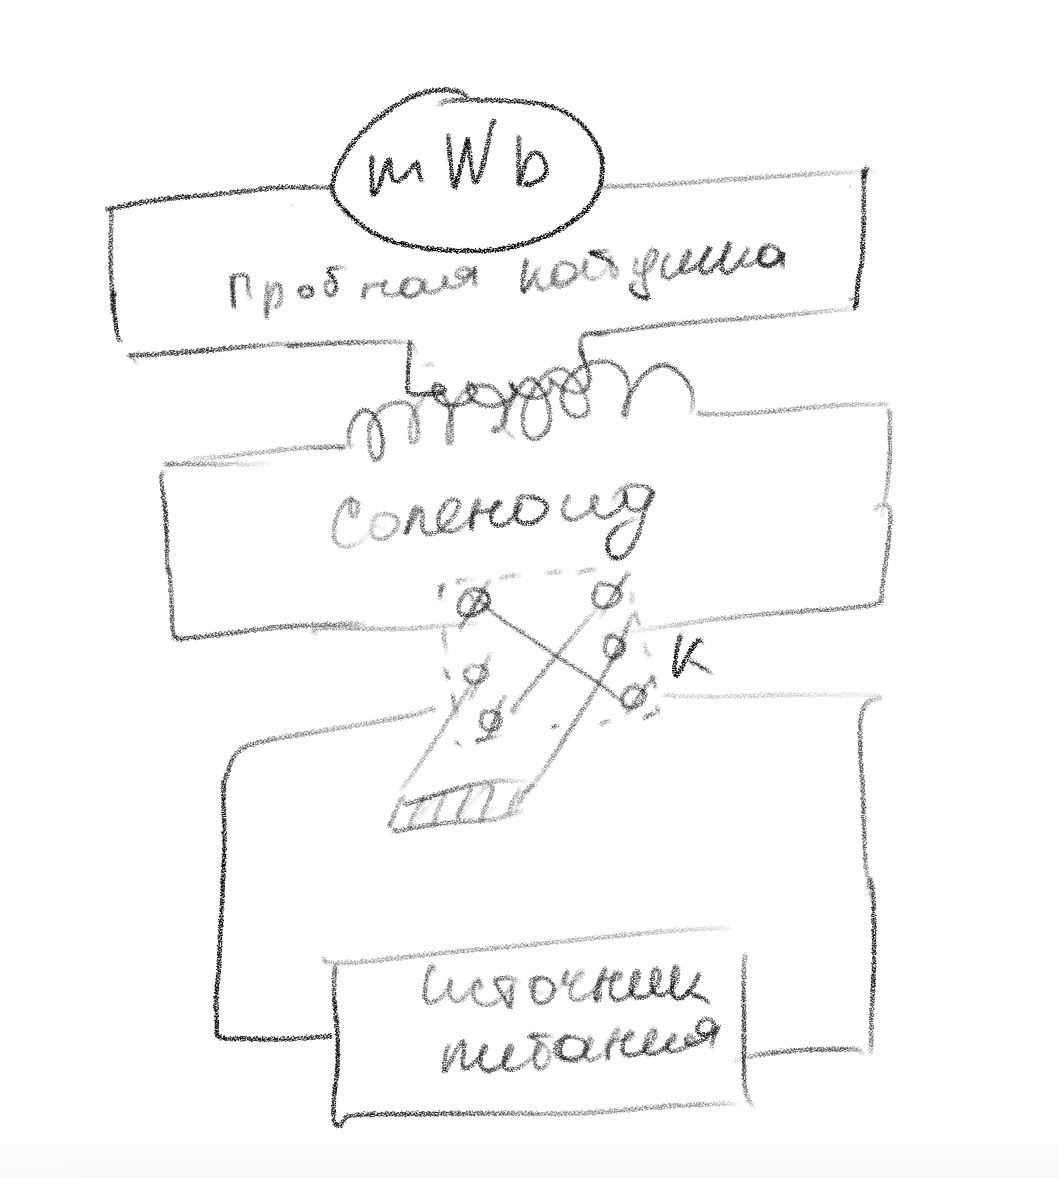
\includegraphics[width=0.7\textwidth]{set}
    \caption{Схема установки}
    \label{fig:set}
\end{figure}
Основной частью установки является электронный осциллограф, трубка которого вынута и установлена в длинном соленоиде, создающим магнитное поле. Напряжение на отклоняющие пластины и питание подводятся к трубке многожильным кабелем.

Пучок электронов, вылетающих из катода с разными скоростями, ускоряется анодным напряжением. Пропустив пучок сквозь две узкие диафрагмы, можно выделить электроны с практически одинаковой продольной скоростью. Небольшое переменное напряжение, поступающее с клеммы "Контрольный сигнал" осциллографа на отклоняющие пластины, изменяет только поперечную составляющую скорости. При увеличении магнитного поля линия на экране стягивается в точку, а затем снова удлиняется. 

Магнитное поле создается постоянным током, величина которого регулируется ручками источника питания и измеряется амперметром. Ключ служит для изменения направления поля в соленоиде.

Величина магнитного поля определяется с помощью милливеберметра.

На точность результатов может влиять внешнее магнитное поле, особенно продольное. 

Измерения магнитного поля с помощью милливеберметра обычно проводятся в предварительных опыта: при отключении ключа устанавливается связь между силой тока и индукцией магнитного поля в соленоиде. 

\subsection{Теоретические сведения}

Удельный заряд электрона определяется по формуле
\begin{equation}
\dfrac{e}{m_e} = \dfrac{8\pi^2V}{l^2} \left(\dfrac{n^2}{B_{\text{ф}}^2} \right),
\end{equation}
где $V$ - ускоряющий потенциал в электронной трубке, $l$ - путь электрона, $B_{\text{ф}}$ - фокусирующее поле, $n$ - номер фокуса.

\subsection{Обработка результатов}
Приведем сведения об установке:
\begin{table}[H]
	\centering
	\begin{tabular}{|c|c|}
	\hline
	Величина & Значение \\ \hline
	l, \text{м}     & 0,265    \\ \hline
	SN, $\text{м}^2$  & 0,3      \\ \hline
	0,116    & 1,8      \\ \hline
	\end{tabular}
	\caption{Данные установки}
	\label{tab:data}
	\end{table}

Данные, полученные во время опыта занесем в таблицу:

\begin{table}[H]
	\centering
	\begin{tabular}{|ccc|ccc|}
	\hline
	\multicolumn{3}{|c|}{В прямом направлении}                                   & \multicolumn{3}{c|}{В обратном направлении}                                     \\ \hline
	\multicolumn{1}{|c|}{I, A (Калибровка)} & \multicolumn{1}{c|}{I, A} & Ф, мВб & \multicolumn{1}{c|}{I, A (Калибровка)} & \multicolumn{1}{c|}{I, A} & Поток, мВб \\ \hline
	\multicolumn{1}{|c|}{0,64}              & \multicolumn{1}{c|}{0,80} & 0,85   & \multicolumn{1}{c|}{4,18}              & \multicolumn{1}{c|}{4,75} & 0,85       \\ \hline
	\multicolumn{1}{|c|}{1,34}              & \multicolumn{1}{c|}{1,60} & 1,60   & \multicolumn{1}{c|}{3,51}              & \multicolumn{1}{c|}{3,69} & 1,70       \\ \hline
	\multicolumn{1}{|c|}{2,06}              & \multicolumn{1}{c|}{2,39} & 2,60   & \multicolumn{1}{c|}{2,80}              & \multicolumn{1}{c|}{3,18} & 2,50       \\ \hline
	\multicolumn{1}{|c|}{2,77}              & \multicolumn{1}{c|}{3,17} & 3,40   & \multicolumn{1}{c|}{2,10}              & \multicolumn{1}{c|}{2,38} & 3,30       \\ \hline
	\multicolumn{1}{|c|}{3,47}              & \multicolumn{1}{c|}{4,06} & 4,20   & \multicolumn{1}{c|}{1,32}              & \multicolumn{1}{c|}{1,58} & 4,00       \\ \hline
	\multicolumn{1}{|c|}{4,14}              & \multicolumn{1}{c|}{4,89} & 4,90   & \multicolumn{1}{c|}{0,60}              & \multicolumn{1}{c|}{0,80} & 5,00       \\ \hline
	\end{tabular}
	\caption{Данные}
	\label{tab:data_data}
	\end{table}

\section{Приложение}



\end{document}